%% SW design: klassebeskrivelse devkit domain klasser
\newpage

\begin{figure}[htbp] \centering
{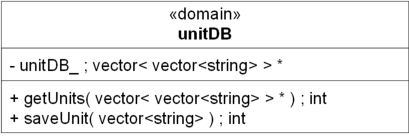
\includegraphics[scale=1.5]{filer/design/Klassediagrammer/sw_unitDB}}
\caption{klassediagram unitDB}
\label{fig:unitDB klassediagram}
\end{figure} 

{\centering
\textbf{unitDB}\par
}
\textbf{Ansvar:} at styre forløbet i UC1: Tilføj / fjern enhed. \

int getUnits( \& int array, \& int size ) \\
\textbf{Parametre:}  \\
\textbf{Returværdi:} 0 ved succes ellers negativ i overenstemmelse med fejl-listen \\
\textbf{Beskrivelse:} \\

int saveUnit( int adresse, int nr ) \\
\textbf{Parametre:}  \\
\textbf{Returværdi:} 0 ved succes ellers negativ i overenstemmelse med fejl-listen \\
\textbf{Beskrivelse:} .\\

\begin{figure}[htbp] \centering
{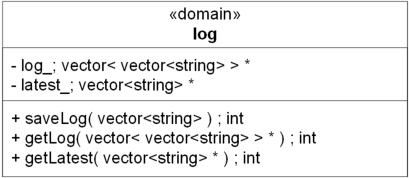
\includegraphics[scale=1.5]{filer/design/Klassediagrammer/sw_log}}
\caption{klassediagram log}
\label{fig:log klassediagram}
\end{figure} 

{\centering
\textbf{log}\par
}
\textbf{Ansvar:} Gemme information loggen til senere brug. \

int saveLog( vector<string> ) \\
\textbf{Parametre:} Modtager en vector af typen string. \\
\textbf{Returværdi:} 0 ved succes ellers negativ i overenstemmelse med fejl-listen \\
\textbf{Beskrivelse:} Modtager log fra enhed og skriver den over i den samlede log og gemmer den i latest \\

int getLog( \& vector<string> )  \\
\textbf{Parametre:} Modtager en adresse til en vector af typen string. \\
\textbf{Returværdi:} 0 ved succes ellers negativ i overenstemmelse med fejl-listen \\
\textbf{Beskrivelse:} .\\

int getLatest( \& vector<string> ) \\
\textbf{Parametre:} Modtager en adresse til en vector af typen string.  \\
\textbf{Returværdi:} 0 ved succes ellers negativ i overenstemmelse med fejl-listen \\
\textbf{Beskrivelse:} .\\


